The Digilent ZedBoard is a developement Platform for the Xilinx Zynq \gls{soc}.
It features a dual-core ARM Cortex-A9 MPCore with a clock-frequency of up to
$866 Mhz$, external memory support, USB and Gigabit Ethernet interfaces as
\gls{ps} and \gls{pl} based on the Xilinx Artix-7 \gls{fpga} series.
The \gls{pl} can be used stand-alone, but the \gls{ps} is dependent on the
\gls{pl}.

For this project, the \gls{pl} needs to be configured with peripherals for the
processor that are needed by the Linux kernel as well as the hardware
accelerators.
The resulting system must then be partitioned for the dynamic partial
reconfiguration.
This is discussed in \Cref{ssec:zynqhardwaredesign}.

The \gls{ps} needs to be configured with all the software that Android needs to
boot, to interact with the hardware accelerators and to dynamically reconfigure
the \gls{pl}.
This is done in \Cref{ssec:zynqsoftwaredesign}.

The complete design is available as a git repository at~\cite{repo}.
File paths within this document may refer to the root directory of the git
repository by using \emph{<repo>}.
To interact with the ZedBoard, multiple interfaces are used:
\begin{itemize}
	\item A command line interface is available over an \gls{uart} interface
	\item Ethernet is used to access the internet
	\item Graphical output is available over a \gls{hdmi}
	\item Peripherals can be attached via \gls{otg}
\end{itemize}
To achieve the best android experience, a touchscreen is attached via \gls{hdmi}
(for graphics) and \gls{otg} (for the \gls{hid}).

To automate the extensive build process, two scripts are available in our git
repository.
\emph{<repo>/bootimage/generate\_without\_android.sh} compiles the bitstream,
\gls{fsbl}, u-boot, the linux kernel and the kernel modules.
Android is built seperately, since it requires a special build environment that
not all members of the team had access to.
To build android, the script
\emph{<repo>/bootimage/generate\_including\_android.sh} can be executed.

Both scripts rely on makefiles of the underlying components they are building.
This means that components that were not changed since the last build are not
going to be recompiled.
This saves build time during development.
\subsection{Zynq Hardware Design}\label{ssec:zynqhardwaredesign}
In contrast to the previous project \cite{oldrepo}, no hardware design was provided. Therefore, the hardware design had to be created. The reference design \cite{TRDReferenceDesign} from Xilinx served as a template. It includes all the peripherals that are needed by the Linux kernel to run on the ZCU102 Evaluation Kit.


Digilent provides a reference design~\cite{DigilentReferenceDesign} that
includes all the peripherals that are needed by the linux kernel to run on the
ZedBoard.
This is the design that is used to build the boot-image flashed onto the SD
card that comes with the ZedBoard.
It contains a \gls{xps} Project that can be opened and built using
the corresponding \emph{xps} tool that is included in the Xilinx ISE Design
Suite.
Digilent claims that they used version \emph{14.4}. Unfortunately, that version
is missing the \emph{axi\_vdma} core in revision \emph{v5\_01\_a}.
That particular revision was removed in \emph{ISE 14.4} but is available in
\emph{ISE 14.1} and replace with a newer version.
Without the knowledge of the old version, the Xilinx tools are unable to upgrade
the core to the new revision.

To mitigate this issue, both versions of \emph{ISE} were installed and the core
was imported from the old version to the new version using a symbolic link.
This allowed us to build the project in \emph{ISE 14.4}.
Since the support for \gls{dpr} is better in \emph{ISE 14.7}, we chose to use
that version.

To import the old \emph{axi\_vdma} core into the new version of \emph{ISE}, the
command in \Cref{lst:corelink} can be used, assuming \emph{ISE} was installed in
the default directory \emph{/opt}.
\begin{lstlisting}[
	language=Bash,
	caption={Link \emph{axi\_vdma} core from \emph{ISE 14.1} to \emph{14.4}},
	label={lst:corelink},
	basicstyle=\small,
	float=h,
	floatplacement=h
	]
	ln -s /opt/Xilinx/14.1/ISE_DS/EDK/hw/XilinxProcessorIPLib/pcores/axi_vdma_v5_01_a /opt/Xilinx/14.7/ISE_DS/EDK/hw/XilinxProcessorIPLib/pcores/axi_vdma_v5_01_a
\end{lstlisting}

This design can then be adapted to include our logic needed for the hardware
accelerators.
Digilent published a tutorial~\cite{DigilentTutorial} on how to do this on a
simple example.
The basic steps to do this are:
\begin{itemize}
	\item Create new peripheral by choosing `Hardware', `Create or Import
		Peripheral\ldots'
	\item The new peripheral can now be found in the `Project Local PCores'
		under the `USER' registry.
		Add it to the design by right clicking on it and choosing `Add IP'
	\item Add it to the Zynq Processing System when prompted to do so
	\item Assign an address and memory size in the `Addresses' tab
\end{itemize}
For the last step, choose a free address.
The address-table for the included devices is configured as follows:

\begin{tabular}{llll}
	Instance                & Base Address & High Address & Size\\
	processing\_system7\_0  & 0x00000000   & 0x1FFFFFFF   & 512M\\
	axi\_dma\_0             & 0x40400000   & 0x4040FFFF   & 64K\\
	axi\_iic\_0             & 0x41600000   & 0x4160FFFF   & 64K\\
	axi\_vdma\_0            & 0x43000000   & 0x4300FFFF   & 64K\\
	axi\_hdmi\_tx\_16b\_0   & 0x70E00000   & 0x70E0FFFF   & 64K\\
	axi\_spdif\_tx\_0       & 0x75C00000   & 0x75C0FFFF   & 64K\\
	axi\_clkgen\_0          & 0x79000000   & 0x7900FFFF   & 64K
\end{tabular}

The custom logic cores can be assigned addresses starting from $0x7E400000$.

\gls{xps} generates two \gls{vhdl} files for the core.
One is called `user\_logic.vhd' and the other carries the name of the core
itself.
The first one contains the actual logic.
The tool generates a simple interface so that the logic can react to register
reads and writes.
The second file maps that simple interface to the \gls{axi} interface so that
it can be connected to Zynq's \gls{axi} bus.

The complete hardware design is available as a \gls{xps} project in the git repo
at \emph{<repo>/hardware\_design/system.xmp}.

The logic design of the two hardware accelerators is discussed in the following
subsections.

\subsubsection{Blake2B Module}\label{sssec:blake2bmodule}
Blake2~\cite{blake2} is a cryptographic hash and \gls{mac}. It is faster than
\emph{MD5}, \emph{SHA-1}, \emph{SHA-2} and \emph{SHA-3}, but is at least as
secure as the latest standard \emph{SHA-3}.
It comes in two flavors:
\begin{itemize}
	\item \emph{Blake2B} is optimized for $64$-bit platforms and produces
		digests of any size between $1$ and $64$ bytes
	\item \emph{Blake2S} is optimized for $8$- to $32$-bit platforms and
		produces digests of any size between $1$ and $32$ bytes.
\end{itemize}

A hardware implementation was created by Benedikt Tutzer and Dinka Milovancev as
part of the \emph{Digital Integrated Circuits} Laboratory at TU
Wien~\cite{blake2hardware}.
Even though we are working on a $32$-bit platform, we chose to implement
Blake2B, since at hardware level we can chose what bit-width to use.

The core is added to the system design as described in
\Cref{ssec:zynqhardwaredesign} and given the address $0x7E410000$. A size of
$64K$ is sufficient.
\gls{xps} generates the needed files in
\emph{<repo>hardware\_design/pcores/blake2b\_v1\_00\_a}.
The files from~\cite{blake2hardware} are then added to the vhdl-source directory
of the core,\\
\emph{<repo>/hardware\_design/pcores/blake2b\_v1\_00\_a/hdl/vhdl}.
\gls{xps} needs to be made aware of the additional files, otherwise they will be
left out of the synthesis flow.
To include them, the \gls{pao} file of the core, found in
\emph{<repo>/hardware\_design/pcores/blake2b\_v1\_00\_a/data/blake2b_v2_1_0.pao},
needs to be adapted accordingly (\Cref{lst:blake2,lst:blake2bwrapper}):

\begin{lstlisting}[
	language=Bash,
	caption={\gls{pao} file of the blake2b core},
	label={lst:mpdblake},
	basicstyle=\small,
	float=h,
	floatplacement=h
	]
lib proc_common_v3_00_a  all 
lib axi_lite_ipif_v1_01_a  all 
lib blake2b_v1_00_a blake2 vhdl(*@\label{lst:blake2}@*)
lib blake2b_v1_00_a blake2b_wrapper vhdl(*@\label{lst:blake2bwrapper}@*)
lib blake2b_v1_00_a user_logic vhdl
lib blake2b_v1_00_a blake2b vhdl
\end{lstlisting}

The entity from~\cite{blake2hardware} needs to be wrapped in the user\_logic.vhd
file.
It was configured to have $4$ software accessible registers, each $32$-bit wide:

\begin{tabular}{ll}
	Address & Name \\
	base     & task\_reg\\
	base + 4 & message\_reg\\
	base + 8 & status\_reg\\
	base + 16 & hash\_reg\\
\end{tabular}

With interface generated by the Xilinx tools, the core is only able to react to
register reads or -writes from the software.
It cannot send interrupt to the software.
To add this functionality, an additional port, of type \emph{std\_logic} is
added and routed through the wrapper in \emph{blake2b.vhd} so that it is
visible as an output port of the peripheral.
It is called \emph{Interrupt}.
To have it act as an interrupt signal, it has to be declared as such in the
cores \gls{mpd} file,
\emph{<repo>/hardware_design/pcores/blake2b_v1_00_a/data/blake2b\_v2\_1\_0.mpd}.
This is done with the following lines:

\begin{lstlisting}[
	language=Bash,
	caption={Configure output port as interrupt},
	label={lst:interruptmpd},
	basicstyle=\small,
	float=h,
	floatplacement=h
	]
PARAMETER C_INTERRUPT_PRESENT = 1, DT = INTEGER, RANGE = (0,1)
PORT Interrupt = "", DIR = O, SIGIS = INTERRUPT, SENSITIVITY = EDGE_RISING, INTERRUPT_PRIORITY = MEDIUM, ISVALID = (C_INTERRUPT_PRESENT == 1)
\end{lstlisting}

The port then shows up as an interrupt port.
To connect it to the \gls{gic}, one must select the Zynq tab and click on the
\emph{IRQ} table as seen in \Cref{fig:gic}.

\begin{figure}[h]
\centering
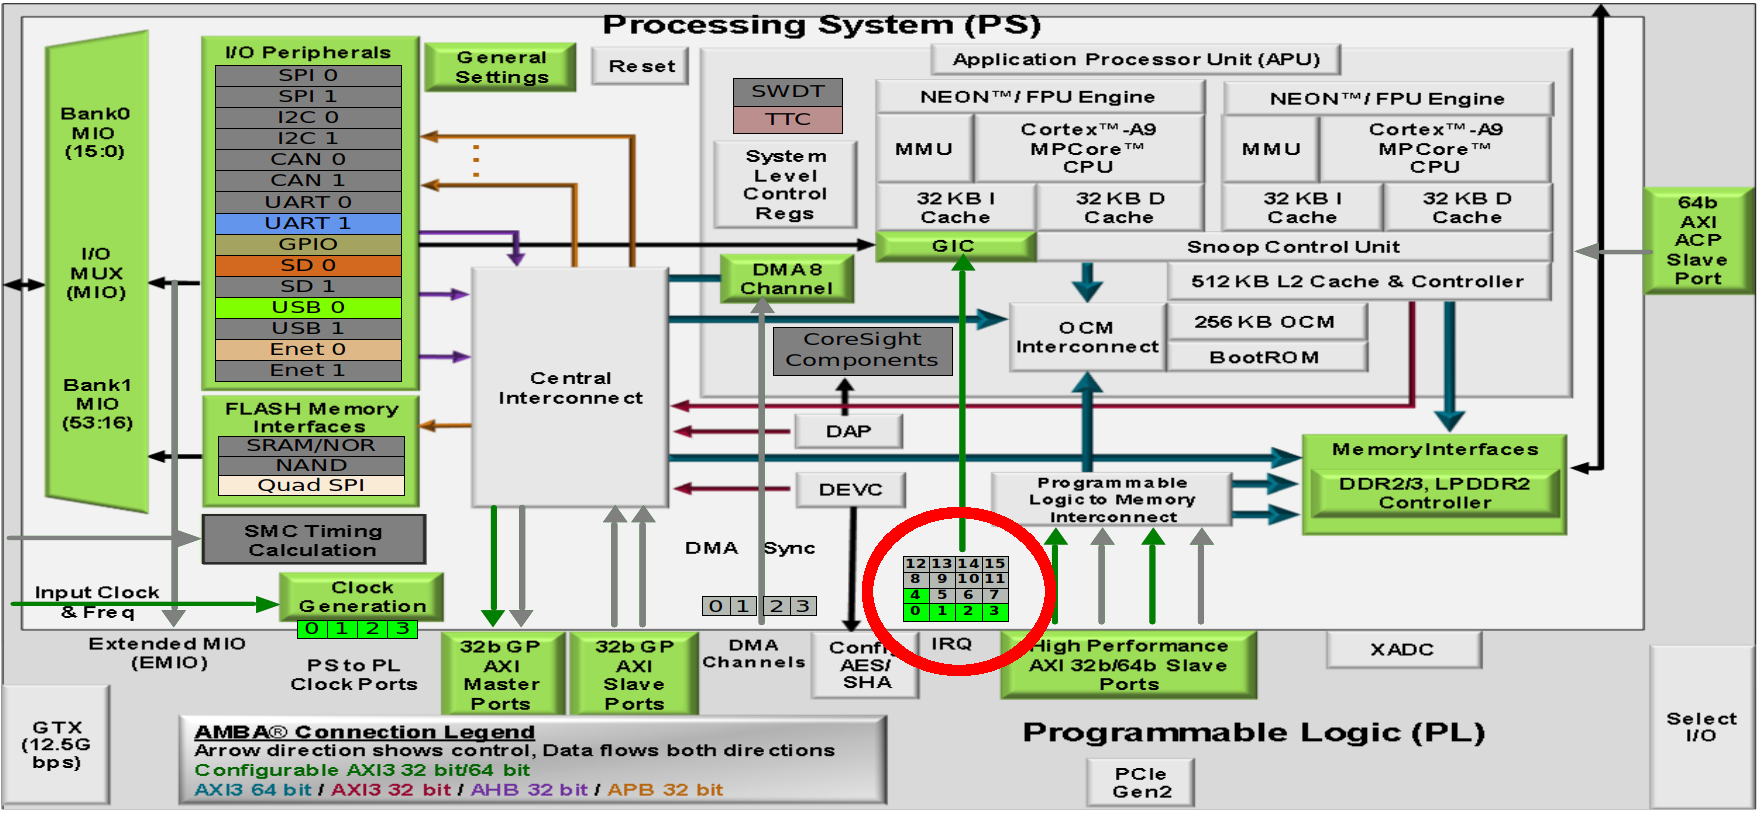
\includegraphics[width=1\textwidth]{sections/methodology/gic}
\caption{\label{fig:gic} IRQ table in the Zynq tab}
\end{figure}

On the upcoming dialog, the interrupt signal is shown as unconnected interrupt
in the left column.
By selecting it and clicking the arrow that points to the right it can be moved
to the right and is then connected, as seen in \Cref{fig:gicconnect}.

\begin{figure}[h]
\centering
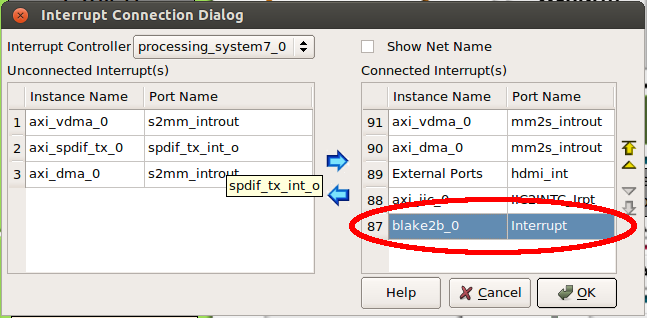
\includegraphics[width=1\textwidth]{sections/methodology/gicconnect}
\caption{\label{fig:gicconnect} Interrupt Connection Dialog}
\end{figure}

The number shown on the left side of the right column, $87$ in this example, is
the interrupt number that the device driver will have to connect to.
This can be seen in \Cref{sssec:linuxkernelmodules}.

The protocol how this device communicates with the device driver is simple.
To hash data, it has to be split into chunks of $32$-bits as the registers are
only $32$ bits wide.
The following steps need to be followed to hash data:
\begin{enumerate}
	\item Driver writes number of bytes to be hashed to the task register
	\item If all the data was sent, go to \Cref{item:end}\label{item:check}
	\item Device raises interrupt to signal that more data is needed
	\item Driver catches interrupt and writes a chunk of data to the message
		register
	\item Go to \Cref{item:check}
	\item Device raises interrupt to signal that hashing is done\label{item:end}
\end{enumerate}
The hash is always $64$-bytes long, so to read it back to the driver it has to
be split into $16$ individual $32$-bit chunks.
To read the hash from the device, the following steps are done:
\begin{enumerate}
	\item Driver iterates over $16$ hash chunks
		\begin{enumerate}
			\item Driver writes index of hash-chunk to status register
			\item Devices places the according chunk onto the hash register
			\item Driver reads hash register
		\end{enumerate}
	\item Driver concatenates hash chunks
\end{enumerate}

\subsubsection{Image Processing Module}\label{sssec:imageprocessingmodule}
The following three types of image filters have been designed:
\begin{itemize}
\item Red-Filter
\item Green-Filter
\item Blue-Filter
\end{itemize}
These simple filters read pixel data from an \gls{axi} interface and filter out
all channels except one.
The red filter filters out everything but the red channel\ldots.
Figure \ref{fig:imagefilter} describes the principle of the filter
functionality.
The logic of these filters is connected to the \gls{axi}-Lite Bus.
All three filters share a common Wrapper-Interface and are accessible by a
common Linux-Device-Driver.\\
\begin{figure}[h]
\centering
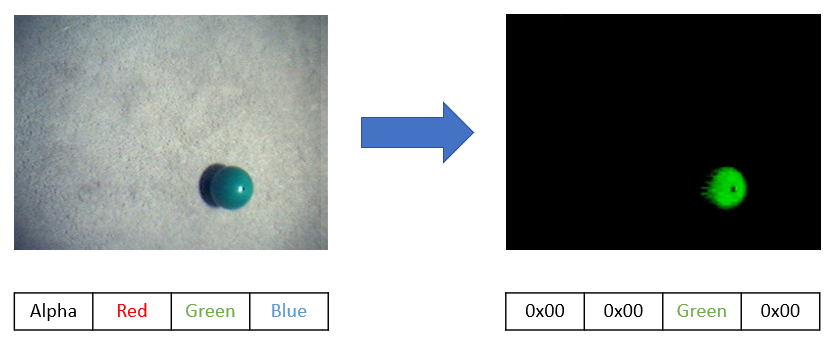
\includegraphics[width=1\textwidth]{sections/methodology/ImageFilter.PNG}
\caption{\label{fig:imagefilter} Green Filter example}
\end{figure}
The different cores are added to the system design via the concept described in
section \ref{sssec:partialreconfigurationsetup} at the address $0x7E430000$ with
the size of $64K$.
The logic behind the common wrapper uses 2 software accesible registers, each
32-bit wide:\\
\begin{tabular}{ll}
	Address & Name \\
	base     & write\_reg\\
	base + 4 & read\_reg\\
\end{tabular}\\
The value of the write\_register is processed by the synthesized filter logic
and the result is written to the read\_register.
The related Linux device driver (\ref{sssec:linuxkernelmodules}) iterates over
the raw \gls{rgb} data written to the device driver file and stores the filtered
data which can then be read back from the device driver file.

\subsubsection{Partial Reconfiguration Setup}\label{sssec:partialreconfigurationsetup}
Partial reconfiguration was done using the planAhead tool included in the Xilinx ISE Design Suite. Compared to the Vivado Design Suite, where \gls{dpr} works with the \gls{vhdl} files, the planAhead tool only works with the synthesized netlists.

For \gls{dpr} a Bottom-Up Synthesis is required. The static logic is synthesized with a black box module definition for each \gls{dpr} module.

The synthesis is done inside the script\\\emph{<repo>/bootimage/generate\_without\_android.sh}. Since the netlists for the different filter logics are not synthesized with the flow, they must be generated separately. Both is done with the following lines: 

\begin{lstlisting}[
	language=Bash,
	caption={Synthesis for project},
	label={lst:makenetlist},
	basicstyle=\small,
	float=h,
	floatplacement=h
	]
make -f system.make netlist
# generate netlists for filter logic
xst -ifn synth_filter_logic.xst
\end{lstlisting}

Xilinx provides a tutorial \cite{planAheadTutorial} that describes how the \gls{dpr} is done with the planAhead tool. First, the \gls{gui} based design was used to create the bitstreams. Afterwards a \gls{tcl} script, \emph{<repo>/hardware_design/planAhead.tcl}, was implemented with the included \gls{tcl} console. This script automatically generates the bitstreams used for partial reconfiguration. \Cref{lst:runplanahead} shows how the planAhead tool can be started in \gls{tcl} mode and start the script.

\begin{lstlisting}[
language=Bash,
caption={Run planAhead in \gls{tcl} mode},
label={lst:runplanahead},
basicstyle=\small,
float=h,
floatplacement=h,
breaklines=true
]
planAhead -mode tcl -source planAhead.tcl
\end{lstlisting}

In our project $6$ bitstreams are generated:
\begin{itemize}
	\item $3$ full bitstreams with different filter logic
	\item $3$ partial bitstreams with different filter logic
\end{itemize}

Before the partial bitstreams can be used, they need to be transformed into an other format. With the following lines the bitstreams are converted:

\begin{lstlisting}[
language=Bash,
caption={Convert bitstreams into binary files},
label={lst:convertbit},
basicstyle=\small,
float=h,
floatplacement=h
]
promgen -b -w -p bin -data_width 32 -u 0 ./planAhead/partial_reconfiguration/partial_reconfiguration.runs/config_1/config_1_simple_filter_0_simple_filter_0_USER_LOGIC_I_filter_logic_0_red_filter_partial.bit -o ./planAhead/generated_Bitstreams/red_filter.bin
promgen -b -w -p bin -data_width 32 -u 0 ./planAhead/partial_reconfiguration/partial_reconfiguration.runs/config_2/config_2_simple_filter_0_simple_filter_0_USER_LOGIC_I_filter_logic_0_green_filter_partial.bit -o ./planAhead/generated_Bitstreams/green_filter.bin
promgen -b -w -p bin -data_width 32 -u 0 ./planAhead/partial_reconfiguration/partial_reconfiguration.runs/config_3/config_3_simple_filter_0_simple_filter_0_USER_LOGIC_I_filter_logic_0_blue_filter_partial.bit -o ./planAhead/generated_Bitstreams/blue_filter.bin
\end{lstlisting}

\subsection{Zynq Software Design}\label{ssec:zynqsoftwaredesign}
The Zynq Software Design consists of the following components:
\begin{itemize}
	\item The \gls{fsbl}
	\item The \emph{u-boot} utility
	\item A linux kernel
	\item The Android Operating System
	\item Linux kernel modules
	\item The image processing app
\end{itemize}
Setting up the \gls{fsbl} and the u-boot utility is described in detail
in~\cite{DigilentTutorial}.
The only important thing to note is that u-boot needs to be built from source
code revision \emph{b55d4b1}, as the support for the ZedBoard changed
afterwards.
\cite{DigilentTutorial} also provides instructions on how to build the linux
kernel, but since we need it to be able to boot Android quite some modifications
were needed so it is explained in detail in \Cref{sssec:linuxonzedboard}.
The Android setup itself is discussed in \Cref{sssec:androidonzedboard}, while
\Cref{sssec:linuxkernelmodules} talks about the kernel modules and
\Cref{sssec:imageprocessingapp} details the Android app.
Finally, \Cref{sssec:dynamicpartialreconfiguration} talks about how we set up
the software system to be able to do \gls{dpr}.

\subsubsection{Linux on ZedBoard}\label{sssec:linuxonzedboard}
Digilent provides a branch of the linux kernel that is compatible with most of
their boards, including the ZedBoard~\cite{DigilentLinux}.
Source revision \emph{06b3889} was found to be the most recent to include
android support.

To build linux from~\cite{DigilentLinux} for the ZedBoard with Android support,
the following steps need to be followed:
\begin{enumerate}
	\item \emph{Fix the device tree} by copying the device tree from
		\cite{DigilentReferenceDesign} to
		\emph{<kernel>/arch/arm/boot/dts/digilent-zed.dts}
	\item \emph{Setup build environment to use Xilinx tools} by setting
		environment variables as seen in \Cref{lst:envsetup}
	\item \emph{Generate default configuration for the ZedBoard} by running
		\emph{make digilent\_zed\_defconfig}
	\item \emph{Add Android and touchscreen related configurations} by running
		\emph{make menuconfig}
		\begin{enumerate}
			\item Navigate to `Device Drivers' and enable `Staging Drivers'
			\item Navigate to `Device Drivers' `Staging Drivers', `Android'
				and enable all entries
			\item Navigate to `Device drivers', `Input device support' and
				enable `Touchscreens'
			\item Navigate to `Device drivers', `Input device support',
				`Touchscreens' and enable
				\begin{itemize}
					\item `Ilitek ILI210X based touchscreen'
					\item `USB Touchscreen Driver'
				\end{itemize}
			\item Navigate to `Device drivers', `HID support', `Special HID
				drivers' and enable `HID Multitouch panels'
		\end{enumerate}
	\item \emph{Build the kernel} by running \emph{make}
	\item \emph{Build the device tree} by running \emph{./scripts/dtc/dtc -I dts
		-O dtb -o devicetree.dtb arch/arm/boot/dts/digilent-zed.dts}
\end{enumerate}
\begin{lstlisting}[
	language=Bash,
	caption={Environment setup to build the linux kernel},
	label={lst:envsetup},
	basicstyle=\small,
	float=htbp,
	floatplacement=htbp
	]
export CCOMPILER=arm-xilinx-linux-gnueabi-gcc
export ARCH=arm
export CROSS_COMPILE=arm-xilinx-linux-gnueabi-
export PATH=$PATH:/opt/Xilinx/14.7/ISE_DS/EDK/gnu/arm/lin/bin/		
\end{lstlisting}
The compiled image will be available in \emph{arch/arm/boot/zImage}.
To boot it requires a ramdisk, available from~\cite{DigilentReferenceDesign}.
To have the linux kernel to load our kernel modules and start Android when the
boot was successul, the ramdisk has to be adapted.
The easiest way to do this is to make the startup script in
\emph{etc/init.d/rcS} execute our own startup scripts from the SD card after
everything else is done.

We created two startup scripts, one to load the kernel modules
(\emph{<repo>/linux-files/startup.sh}) and one to start android
(\emph{<repo>/linux-files/startup\_android.sh}).

\subsubsection{Android on ZedBoard}\label{sssec:androidonzedboard}
Android Gingerbread on ZedBoard was officially supported by Xilinx partner
company Iveia, unfortunately it is not any more and they do not longer provide
android sources. Thankfully, a github user made the Iveia sources available by
uploading them~\cite{androidsource}.

Android Gingerbread requires a very delicate build environment:
\begin{itemize}
	\item Ubuntu 12.04 LTS host operating system
	\item make version 3.81
	\item gcc, g++ and cpp version 4.4
	\item Java JDK 1.6 from Oracle (the OpenJDK version is not suitable)
	\item The following packages available from the Ubuntu repositories:
		apt-get install libgtk2.0-0:i386 libxtst6:i386 gtk2-engines-murrine:i386
		lib32stdc++6 libxt6:i386 libdbus-glib-1-2:i386 libasound2:i386 fakeroot
		build-essential crash kexec-tools makedumpfile kernel-wedge git-core
		libncurses5 libncurses5-dev libelf-dev asciidoc binutils-dev curl
		gcc-4.4 g++-4.4 cpp-4.4 gcc-4.4-multilib g++-4.4-multilib cpp-4.4
		ia32-libs openjdk-6-jdk:i386 vim gnupg flex bison gperf build-essential
		zip curl libc6-dev x11proto-core-dev libx11-dev:i386
		libreadline6-dev:i386 libgl1-mesa-glx:i386 libgl1-mesa-dev g++-multilib
		mingw32 tofrodos python-markdown libxml2-utils xsltproc zlib1g-dev:i386
		gnupg flex bison gperf build-essential zip curl libc6-dev
		lib32ncurses5-dev x11proto-core-dev libx11-dev:i386
		libreadline6-dev:i386 libgl1-mesa-glx:i386 libgl1-mesa-dev
		g++-multilib mingw32 tofrodos python-markdown libxml2-utils xsltproc
		zlib1g-dev:i386 genext2fs lib32z1-dev
	\item The repo tool (a wrapper around git), available from\\
		\url{http://commondatastorage.googleapis.com/git-repo-downloads/repo}
\end{itemize}
The build process can be seen in \Cref{lst:androidbuild}.
\begin{lstlisting}[
	language=Bash,
	caption={Retrieve and build android},
	label={lst:androidbuild},
	basicstyle=\small,
	float=h,
	floatplacement=h
	]
repo init -u git://github.com/aimeemikaelac/xilinx-android-manifest.git -b android-zynq-1.0(*@\label{lst:androidret1}@*)
repo sync(*@\label{lst:androidret2}@*)

. build/envsetup.sh(*@\label{lst:androidenv1}@*)
lunch generic-eng(*@\label{lst:androidenv2}@*)


make -j32(*@\label{lst:androidmake1}@*)
make -f Makefile.zynq(*@\label{lst:androidmake2}@*)

mkdir -p root(*@\label{lst:touchcopy1}@*)
sudo mount root.img -o loop,rw,sync root
sudo mkdir -p root/system/usr/idc/
sudo cp <repo>linux-files/touchscreen_config.idc root/system/usr/idc/Vendor_222a_Product_0001.idc
#sudo cp <repo>/linux-files/touchscreen_config.idc "root/system/usr/idc/ILITEK ILITEK-TP.idc"
sudo chmod 664 root/system/usr/idc/*.idc
sleep 1
sudo umount root
sleep 1
rmdir root(*@\label{lst:touchcopy2}@*)
\end{lstlisting}
In \Crefrange{lst:androidret1}{lst:androidret2} the source code is retrieved.
\Crefrange{lst:androidenv1}{lst:androidenv2} setup the environment and
\Crefrange{lst:androidmake1}{lst:androidmake2} builds the system.
The result is a bootable image called `root.img'.

This image then needs to be mounted, so we can copy the touchscreen
configuration file to it. This is done in
\Crefrange{lst:touchcopy1}{lst:touchcopy2}.

\subsubsection{Linux Kernel Modules}\label{sssec:linuxkernelmodules}

\textbf{Blake2b Driver:}\\
The blake2b device driver sits between the userspace application that desires to
compute the hash of a file and the \gls{pl} implementation of Blake2B.\\
The communication with the \gls{pl} was discussed in detail in
\Cref{sssec:blake2bmodule}.\\
The interface to the userspace application is simple.
The driver creates a device file \emph{/proc/blake2b}.
The userspace application can then write a file path to that file.
This triggers the start of the hashing function.
Afterwards, the application can read $64$ bytes from the device file, these
bytes will contain the hash.\\
The blake2b driver code is available at \emph{<repo>/drivers/blake2b/blake2b.c}.
The code is quite self explanatory and therefore not discussed in detail here.
One caveat is that one has to call the function \emph{wmb} between subsequent
reads or writes to the device.
This function will impede the compiler to rearrange the calls during
optimization and therefore guarantees that the reads and writes are executed in
specified order.
\\\\
\textbf{Image Filter Driver:}\\
The Image Filter device driver writes raw \gls{rgb} data that needs to be
processed to the write register address of the programmed filter logic.
The processing of the value is then triggered automatically.
Afterwards the filter data is read from the read register address by the driver.
The interface to the userspace application is implemented by writing and reading
from a related \emph{.bin} file.
The absolute path of this file has to be communicated to the device driver.

The communication with the \gls{pl} is discussed in section
\ref{sssec:imageprocessingmodule}.
The communication with the application is discussed in section
\ref{sssec:imageprocessingapp}.
The developed driver creates a device file \emph{/proc/simple\_filters}, which
can be triggered by the user application.
The driver code itself is available at\\
\emph{<repo>/drivers/simple\_filters/simple\_filters.c}.

\subsection{Image Processing App}\label{sssec:imageprocessingapp}
The Image processing app splits into two parts. An external server which provides the infrastructure to store and distribute bitstreams and 
the android app (client) which interacts with the server and the hardware on the ZedBoard. 

\subsubsection{Client application}

The client is a native android application written in Android Studio version 3.2.1 for Android API 10 (Gingerbread 2.3.3).
Unfortunately todays Android SDK (API 28) does not support Gingerbread anymore, version 25 was the last SDK that officially supports Gingerbread. To compile for Gingerbread set compileSdkVersion to 25 with the targetSdk set to 10 as seen in~\Cref{lst:appbuild}.
\begin{lstlisting}[
	language=Bash,
	caption={App build setup},
	label={lst:appbuild},
	basicstyle=\small
	]
apply plugin: 'com.android.application'
android {
    compileSdkVersion 25
    defaultConfig {
        applicationId "com.lab.soc.client"
        minSdkVersion 10
        targetSdkVersion 10
        versionCode 1
        versionName "1.0"
        testInstrumentationRunner "android.support.test.runner.AndroidJUnitRunner"
    }
    buildTypes {
        release {
            minifyEnabled false
            proguardFiles getDefaultProguardFile('proguard-android.txt'), 
            'proguard-rules.pro'
        }
    }
    buildToolsVersion '28.0.3'
}

dependencies {
    implementation fileTree(include: ['*.jar'], dir: 'libs')
    implementation 'com.android.support:appcompat-v7:25.4.0'
    implementation 'com.android.support.constraint:constraint-layout:1.1.3'
    implementation 'com.android.support:support-v4:25.4.0'
    testImplementation 'junit:junit:4.12'
    androidTestImplementation 'com.android.support.test:runner:1.0.2'
    androidTestImplementation 'com.android.support.test.espresso:espresso-core:3.0.2'
}    
\end{lstlisting}
This way it is possible to use Google's support libraries, which deliver
backward compatibility for newer Android classes (e.g fragments) and allows to run the app on all Android versions from Gingerbread to Pie without version specific modifications. Whenever possible Androids own APIs has been used, if not available on Gingerbread they were replaced with own implementations.\newline

The architecture is following the single responsibility principle, separating the concerns into several classes:

\begin{itemize}
    \item MainActivity 	    - Android specific (UI, Events, Life cycle)
    \item NetworkManager	- Network operations 
    \item MsgProcessor	    - JSON processing 
    \item FabricManager	    - PL Fabric interaction
    \item AppExecutors	    - Multi threading
    \item Util			    - Utility (Image preprocessing)
    \item Repository        - Data format
\end{itemize}


The Network Manager spawns a new thread and opens a connection to the server. Then requests new information using the REST API (see server section). The received information is packed inside a JSON object (JavaScript Object Notation) and forwarded to the MsgProcessor. Where they are unpacked, compared and saved.

Example JSON object:
\begin{verbatim}
{
    "Index": "SOC-LAB-IOT",
    "Title": "IOT Image Processing",
    "Version": "002",
    "Description": "",
    "Changelog": ["3.11.2018 Primary release", 
                    "4.11.2018 Bug fixing", 
                    "6.11.2018 added stuff"],
    "File": "filter_0_0_4.bin",
    "Date": "6.11.2018",
    "Checksum": "fdg851dfg654dfg6541dfg65514dfghdfg45534terg"
}  
\end{verbatim}



If there is a new version available, the Network Manager will download the new bitstream from the sever using the REST API (see server section). The Fabric Manager will then calculate the hash from the bitstream file on the programmable logic. If they match, the PL fabric will be reconfigured with the downloaded bitstream. In a real world scenario, the whole process would run in the background without user interference. For demonstration purposes a simple user interface was implemented to trigger the download and apply filters on a test picture.

\begin{figure}[htbp]
\centering
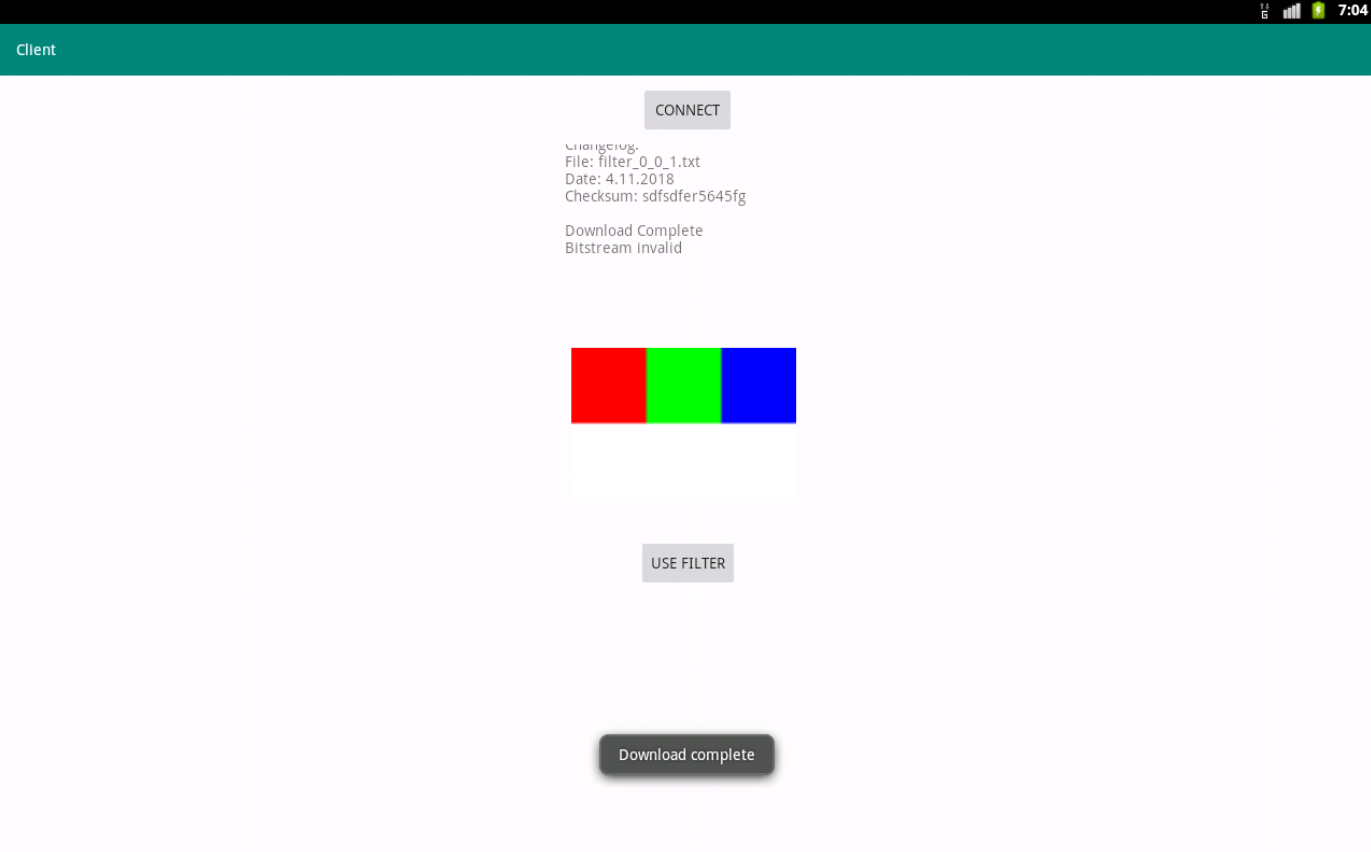
\includegraphics[width=1\textwidth]{sections/methodology/clientdownload.png}
\caption{\label{fig:gui} user interface}
\end{figure}

To apply filters the app has to pre process the image for the device driver to the following specification:
32 bit integer
ALPHA | RED |GREEN | BLUE (8bit|8bit|8bit|8bit) e.g full opaque red would be (hex notation) FF FF 00 00. Every pixel will be read out and saved together to a new binary file. 
The path to this file will be written to the device driver, soon after the filtered data will be read back into the UI from the same file.


\subsubsection{Server}

A tiny webserver with a REST API (Representational State Transfer), 
written with python 3.7 using Flask and its extension FlaskRESTful, therefore fully WSGI compliant
(Webserver Gateway Interface). However Flask internal development server is used for the demonstration and for simplicity.

To start the server, open a terminal in the server directory. Type in following command:
\begin{verbatim}
Flask run -h *your ip* -p 5000    
\end{verbatim}
Open http://*your ip*:5000 to see if the server is reachable

\subsubsection{Server API}

Insomnia, a free open source REST client available for Mac,Windows and Linux, was used for API testing and server communication.

\begin{figure}[htbp]
\centering
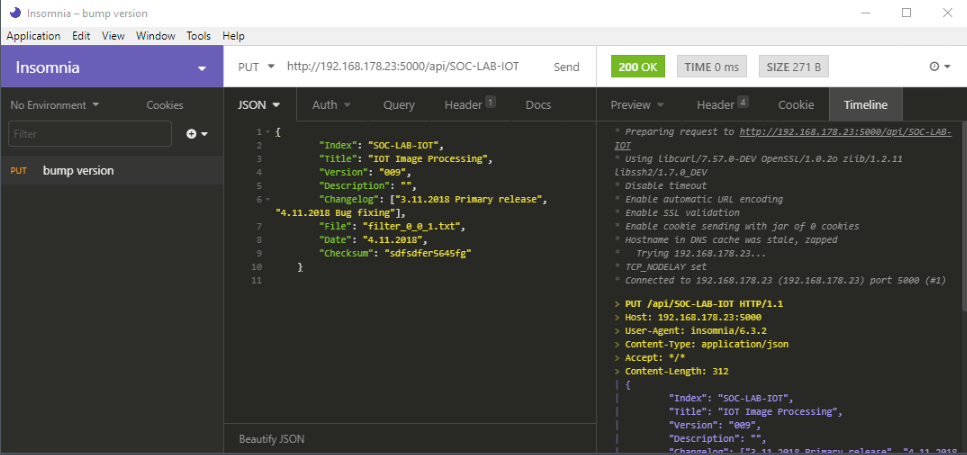
\includegraphics[width=1\textwidth]{sections/methodology/insomnia.png}
\caption{\label{fig:insomnia} Insomnia}
\end{figure}



\newcommand{\specialcell}[2][c]{%
  \begin{tabular}[#1]{@{}c@{}}#2\end{tabular}}
  
\subsubsubsection{Get all information for repository <index>:}
\begin{table}[h]
    \begin{tabular}[h]{llllll}
    URL          & \specialcell{URL\\PARAM}     & \specialcell{DATA\\PARAM}  & METHOD &  \specialcell{SUCCESS\\RESPONSE} & \specialcell{ERROR\\RESPONSE} \\ \hline
    /api/<index> & index=[string] & n/a    & GET   & 200              & 404            \\ 
    \end{tabular}
\end{table}



\subsubsubsection{Create repository <index>:}
\begin{table}[h]
    \begin{tabular}[h]{llllll}
    URL          & \specialcell{URL\\PARAM}     & \specialcell{DATA\\PARAM}  & METHOD &  \specialcell{SUCCESS\\RESPONSE} & \specialcell{ERROR\\RESPONSE} \\ \hline
    /api/<index> & index=[string] & JSON    & POST   & 201              & 400            \\ 
    \end{tabular}
\end{table}

JSON:
\begin{verbatim}
{
    "Index": "SOC-LAB-IOT",
    "Title": "IOT Image Processing",
    "Version": "001",
    "Description": "",
    "Changelog": ["3.11.2018 Primary release", "4.11.2018 Bug fixing"],
    "File": "filter_0_0_1.txt",
    "Date": "4.11.2018",
    "Checksum": ""
}	    
\end{verbatim}

\subsubsubsection{Update repository <index> or create it if not existing:}
\begin{table}[h]
    \begin{tabular}[h]{llllll}
    URL          & \specialcell{URL\\PARAM}     & \specialcell{DATA\\PARAM}  & METHOD &  \specialcell{SUCCESS\\RESPONSE} & \specialcell{ERROR\\RESPONSE} \\ \hline
    /api/<index> & index=[string] & JSON  & PUT    & 200              & 201            \\ 
    \end{tabular}
\end{table}

JSON:
\begin{verbatim}
{
    "Index": "SOC-LAB-IOT",
    "Title": "IOT Image Processing",
    "Version": "002",
    "Description": "",
    "Changelog": ["3.11.2018 Primary release", 
    "4.11.2018 Bug fixing", 
    "6.11.2018 added stuff"],
    "File": "filter_0_0_4.bin",
    "Date": "6.11.2018",
    "Checksum": "fdg851dfg654dfg6541dfg65514dfghdfg45534terg"
}	
\end{verbatim}

\subsubsubsection{Delete repository <index>:}
\begin{tabular}[h]{llllll}
URL          & \specialcell{URL\\PARAM}     & \specialcell{DATA\\PARAM}  & METHOD &  \specialcell{SUCCESS\\RESPONSE} & \specialcell{ERROR\\RESPONSE} \\ \hline
/api/<index> & index=[string] & n/a        & DELETE & 200              & 404            \\ 
\end{tabular}

\subsubsubsection{Download file <filename>}
\begin{tabular}[h]{llllll}
URL          & \specialcell{URL\\PARAM}     & \specialcell{DATA\\PARAM}  & METHOD &  \specialcell{SUCCESS\\RESPONSE} & \specialcell{ERROR\\RESPONSE} \\ \hline
\specialcell{/api/download/\\<path:filename>} &  filename=[string] & n/a        & GET    & 200              & 404            \\ 
\end{tabular}

\subsection{Setup}\label{ssec:setup}
To setup the hardware, one can either:
\begin{itemize}
	\item Build the design himself as described in the previous sections
	\item Use the binaries provided in \emph{<repo>/build}
\end{itemize}
An SD card of at least $4GB$ needs to be formatted as FAT32 and contain the
following files:
\begin{itemize}
	\item \emph{BOOT.BIN}: Contains the \gls{fsbl}, u-boot and the bistream
		for the \gls{pl}
	\item \emph{zImage}: The linux kernel
	\item \emph{root.img}: The Android Operating System
	\item \emph{devicetree.dtb}: The compiled devicetree
	\item \emph{blake2b.ko}: The kernel module for the hashing device
	\item \emph{image\_filter.ko}: The kernel module for the image filters
	\item \emph{ramdisk8M.image.gz}: The ramdisk
	\item \emph{startup.sh}: The script that loads the kernel modules
	\item \emph{startup\_android.sh}: The script that starts Android. If this
		file is missing the boot process will only boot the linux kernel
\end{itemize}
The jumpers on the ZedBoard must be set up as follows:

\begin{center}
	\begin{tabular}{lc}
		JP1 & open\\
		JP2 & short\\
		JP3 & short\\
		JP4 & (open / not populated)\\
		JP5 & (open / not populated)\\
		JP6 & short\\
		JP7 & GND\\
		JP8 & GND\\
		JP9 & 3V3\\
		JP10 & 3V3\\
		JP11 & GND\\
		JP12 & open\\
		JP13 & open\\
		JP18 & 1V8\\
	\end{tabular}
\end{center}
A USB hub can be connected at the \gls{otg} connector.
This can then host a USB Keyboard and the USB touchscreen connector
A \gls{uart} interface is available at the \gls{uart} USB port.
The SD card needs to be inserted into the SD card slot (on the backside of
the ZedBoard, under the FMC connector).
An Ethernet cable can be connected to the Ethernet port.
This can be seen in \Cref{fig:zedboardsetup}.

\begin{figure}[h]
\centering
\includegraphics[width=1\textwidth]{sections/methodology/zedboardsetup}
\caption{\label{fig:zedboardsetup} ZedBoard setup}
\end{figure}

Once everything is set up, the power switch can be switched to the \emph{ON}
position and Android will boot.
After boot, Android will present itself on the display and show the launcher
as seen in \Cref{fig:androiddisplay}.

\emph{NOTE:} The screen must be connected before boot, otherwise the Android
\gls{gui} will not show.

\begin{figure}[h]
\centering
\includegraphics[width=1\textwidth]{sections/methodology/androiddisplay}
\caption{\label{fig:androiddisplay} Android launcher on the ZedBoard display}
\end{figure}

\subsubsection{Dynamic Partial Reconfiguration in Android}\label{sssec:dynamicpartialreconfiguration}
The branch of the Linux kernel provided by Digilent \cite{DigilentLinux} already included a device driver for partial reconfiguration.

Before the driver can be used, it must be set up during the boot routine. \Cref{lst:setuppr} shows how to set up the device driver. In \Cref{lst:ispart} the flag for partial reconfiguration is set.

\begin{lstlisting}[
language=Bash,
caption={Setup partial reconfiguration driver},
label={lst:setuppr},
basicstyle=\small,
float=h,
floatplacement=h
]
echo "++ Adding partial reconfiguration device node"
mknod /dev/xdevcfg c 259 0
echo "1" > /sys/devices/axi.0/f8007000.devcfg/is_partial_bitstream(*@\label{lst:ispart}@*)
\end{lstlisting}

From Android, \gls{dpr} can be easily done by sending the partial bitstream to the device driver. \Cref{lst:prandroid} shows how this is implemented.

\begin{lstlisting}[
language=Bash,
caption={Partial reconfiguration out of Android},
label={lst:prandroid},
basicstyle=\small,
float=h,
floatplacement=h
]
cat new_bitstream.bin > /dev/xdevcfg
\end{lstlisting}

After the reconfiguration is completed, the new logic part can be used.

